%%%%%%%%%%%%%%%%%%%%%%%%%%%%%%%%%%%%%%%%%%%%%%%%%%%
%% LaTeX book template                           %%
%% Author:  Amber Jain (http://amberj.devio.us/) %%
%% License: ISC license                          %%
%%%%%%%%%%%%%%%%%%%%%%%%%%%%%%%%%%%%%%%%%%%%%%%%%%%

\documentclass[a4paper,11pt]{book}
\usepackage[T1]{fontenc}
\usepackage[utf8]{inputenc}
\usepackage{lmodern}

%%%%%%%%%%%%%%%%%%%%%%%%%%%%%%%%%%%%%%%%%%%%%%%%%%%%%%%%%
% Source: http://en.wikibooks.org/wiki/LaTeX/Hyperlinks %
%%%%%%%%%%%%%%%%%%%%%%%%%%%%%%%%%%%%%%%%%%%%%%%%%%%%%%%%%
\usepackage{hyperref}
\hypersetup{unicode=true} % Прибирає hyperref Warning 


\usepackage{graphicx}
\usepackage[ukrainian]{babel}

\usepackage[acronym, toc]{glossaries}

%%%%%%%%%%%%%%%%%%%%%%%%%%%%%%%%%%%%%%%%%%%%%%%%%%%%%%%%%%%%%
% Файли бібліографій                                        %
% Для кожного розділу треба додати строку:                  %
%   \addbibresource{Bibliographies/bib_<номер розділу>.bib} %
%  та відповідний файл в папці Bibliographies/              %
%  куди додавати посилання, експортовані з інших баз даних. %
%%%%%%%%%%%%%%%%%%%%%%%%%%%%%%%%%%%%%%%%%%%%%%%%%%%%%%%%%%%%%
\usepackage[backend=biber,style=numeric,natbib=true]{biblatex}
\addbibresource{Bibliographies/bib_01.bib}
\addbibresource{Bibliographies/bib_02.bib}
\addbibresource{Bibliographies/bib_03.bib}
\addbibresource{Bibliographies/bib_04.bib}




%%%%%%%%%%%%%%%%%%%%%%%%%%%%%%%%%%%%%%%%%%%%%%%%
% Chapter quote at the start of chapter        %
% Source: http://tex.stackexchange.com/a/53380 %
%%%%%%%%%%%%%%%%%%%%%%%%%%%%%%%%%%%%%%%%%%%%%%%%
\makeatletter
\renewcommand{\@chapapp}{}% Not necessary...
\newenvironment{chapquote}[2][2em]
  {\setlength{\@tempdima}{#1}%
   \def\chapquote@author{#2}%
   \parshape 1 \@tempdima \dimexpr\textwidth-2\@tempdima\relax%
   \itshape}
  {\par\normalfont\hfill--\ \chapquote@author\hspace*{\@tempdima}\par\bigskip}
\makeatother

%%%%%%%%%%%%%%%%%%%%%%%%%%%%%%%%%%%%%%%%%%%%%%%%%%%
% Перша сторінка книги, що містить                %
%  - Заголовок та підзаголовок                    %
%  - Ім'я авторів                                 %
%%%%%%%%%%%%%%%%%%%%%%%%%%%%%%%%%%%%%%%%%%%%%%%%%%%

% Заголовок та підзаголовок
\title{\Huge \textbf{Лапароскопічна хірургія печінки}  
\\ \huge Ілюстрований посібник }
% Автор
%\author{\textsc{First-name Last-name}}
\author{
  LastName1, FirstName1
  \and
  LastName2, FirstName2
  \and
  LastName2, FirstName2
  \and
  LastName2, FirstName2
}
\date{}
%%%%%%%%%%%%%%%%%%%%%%%%%%%%%
% Файл глоссарію            %
%(єдиний для всіх розділів) %
%%%%%%%%%%%%%%%%%%%%%%%%%%%%%
\makeglossaries

\newacronym{llr}{ЛРП}{Лапароскопічна резекція печінки}

\newacronym{hals}{ХАРП}{Хенд-ассистована резекція печінки}

\newacronym{hlr}{ГРП}{Гібридна резекція печінки}

\newacronym{olr}{ВРП}{Відкрита резекція печінки}

\newacronym{alr}{АРП}{Анатомічна резекція печінки}

\newacronym{non-alr}{НРП}{Неанатомічна резекція печінки}

\newacronym{llls}{ЛапЛЛС}{Лапароскопічна лівобічна латеральна секцієекомія}

\newacronym{llhe}{ЛапЛГ}{Лапароскопічна лівобічна гемегепатектомія}

\newacronym{lrhe}{ЛапПГ}{Лапароскопічна правобічна гемегепатектомія}

\newacronym{lrps}{ЛапПЗС}{Лапароскопічна правобічна задня секцієекомія}

\newacronym{lras}{ЛапППС}{Лапароскопічна правобічна передня секцієекомія}

\newacronym{lmhe}{ЛапМГЕ}{Лапароскопічна мезогепатектомія}

\newacronym{lce}{ЛапКЕ}{Лапароскопічна каудальна лобектомія}

\newacronym{flr}{МПЗ}{Майбутній печінковий залишок}

\newacronym{bclc}{BCLC}{Barcelona clinic liver cancer staging}

\newacronym{NCCN}{NCCN}{National Comprehensive Cancer Network}

\newacronym{alpps}{ALPPS}{Associating Liver Partition and Portal Vein Ligation for Staged Hepatectomy}

\newacronym{cvp}{ЦВТ}{Центральний венозний тиск}

\newacronym{pdl}{ПДЗ}{Печінково-дванадцятиперсна зв'язка}

\newacronym{ivc}{НПВ}{Нижня порожниста вена}

\newacronym{hv}{ПВ}{Печінкові вени}

\newacronym{lhv}{ЛПВ}{Ліва печінкова вена}

\newacronym{mhv}{СПВ}{Серединна печінкова вена}

\newacronym{rhv}{ППВ}{Права печінкова вена}

\newacronym{hcc}{ГЦК}{Гепатоцеллюлярна карцинома}

\newacronym{crlm}{МКРП}{Метастази колоректального раку в печінку}

\newacronym{nelm}{МНЕП}{Метастази нейроендокринних пухлин в печінку}

\newacronym{btc}{РБТ}{Рак біліарного тракту}

\newacronym{ihcc}{ВПХК}{Внутрішньопечінкова холангіокарцинома}

\newacronym{phcc}{ПХК}{Перихіларна холангіокарцинома}

\newacronym{gbc}{РЖМ}{Рак жовчного міхура}

\newacronym{blt}{ДПП}{Доброякісні пухлини печінки}

\newacronym{hca}{ГЦА}{Гепатоцелюлярна аденома}

\newacronym{fnh}{ФНГ}{Фокальна нодулярна гіперплазія}

\newacronym{hmg}{ГП}{Гемангіома печінки}

\newacronym{bca}{БЦА}{Біліарна цистаденома}

\newacronym{pil}{ПВХ}{Первинний внутрішньопечінковий холелітіаз}

\newacronym{ct}{СКТ}{Спіральна комп'ютерна томографія}

\newacronym{us}{УЗД}{Ультразвукове дослідження}

\newacronym{mri}{МРТ}{Магнітно-резонансна томографія}

\newacronym{icg}{ICG}{Індоціанін зелений}





%%%%%%%%%%%%%%%%%%%%%%%%%%%%%
% Основна частина документа %
%%%%%%%%%%%%%%%%%%%%%%%%%%%%%
\begin{document}

\frontmatter
\maketitle


%%%%%%%%%%%%%%%%%%%%%%%%%%%%%%%%%%%%%
% Auto-generated table of contents, %
%list of figures and list of tables %
%%%%%%%%%%%%%%%%%%%%%%%%%%%%%%%%%%%%%

\tableofcontents
%\listoffigures
%\listoftables

\mainmatter

\clearpage
\printglossary[type=\acronymtype,
               title=Перелік умовних позначеннь]

\newpage

Сучасна хірургія печінки зазнала значних змін завдяки розвитку мінімально інвазивних технологій. Історично, лапароскопічна хірургія розвивалася протягом останніх кількох десятиліть, починаючи з перших експериментальних операцій, які часто супроводжувалися високими ризиками та невизначеністю. Проте, завдяки наполегливій праці хірургів та інженерів, ця методика стала стандартом у провідних клініках світу. Лапароскопічні резекції печінки, які ще двадцять років тому здавалися технічно неможливими, сьогодні вважаються золотим стандартом лікування. Ця трансформація не лише зменшила травматичність операцій, але й значно покращила післяопераційне відновлення пацієнтів, що є критично важливим аспектом у хірургії. Важливість навчання та симуляційних технологій у підготовці нової генерації хірургів не можна переоцінити; ці інструменти дозволяють лікарям отримувати необхідні навички в безпечному середовищі. Автори цієї книги не лише детально описують технічні аспекти операцій, а й розкривають клінічні випадки, що робить книгу надзвичайно цінною для практикуючих хірургів та молодих фахівців. Це видання є унікальним внеском у навчання та практику хірургів, які прагнуть опанувати цей складний, але ефективний метод, надаючи їм необхідні знання для успішного виконання лапароскопічних втручань.

\begin{flushright}
    
\includegraphics[width=0.25\textwidth]{Illustrations/Preface/image1.png} \\
    \textit{Професор Олександр Іванович Петров}
\end{flushright}

\newpage

Видання, яке ви тримаєте в руках, є результатом багаторічного досвіду та глибокого аналізу розвитку лапароскопічної хірургії печінки. У цій книзі автори не тільки узагальнили світовий досвід, а й представили власні досягнення та інноваційні підходи. Порівняння відкритих та лапароскопічних резекцій печінки виявляє численні переваги останніх, включаючи зменшення післяопераційних ускладнень та скорочення термінів госпіталізації. Однак, існують і певні обмеження, які потрібно враховувати. Мій власний досвід впровадження лапароскопічних технологій у хірургічну практику показав, що основними викликами були не лише технічні аспекти, але й необхідність навчання команди та адаптації до нових методик. Сучасні технології, такі як 3D-візуалізація, ICG-навідна резекція та роботизована хірургія, відіграють важливу роль у покращенні безпеки втручань, дозволяючи лікарям виконувати складні операції з максимальною точністю. Ця книга стане незамінним посібником для тих, хто прагне вдосконалити свої навички у сфері сучасної гепатобіліарної хірургії, сприяючи поширенню лапароскопічних резекцій печінки серед хірургів та підвищенню якості лікування пацієнтів.

\begin{flushright}
    
\includegraphics[width=0.25\textwidth]{Illustrations/Preface/image2.png} \\
    \textit{Професор Володимир Сергійович Мельник}
\end{flushright}

\begin{refsection}
\chapter{Введення в лапароскопічну хірургію печінки}
\section{Історія розвитку методики}
\subsection{Перший досвід}
Мініінвазивні втручання радикально змінили хірургічну практику за останні три десятиріччя та призвели до суттєвого покращення результатів за рахунок зменшення частоти післяопераційних ускладненнь, тривалості госпіталізації та співвідношення вартості до еффективності лікування в різних хірургічних спеціальностях, включаючи колоректальну хірургію, урологію, гінекологію та торокальну хірургію. Природньо, що зацікавленість хірургів в лапароскопічному доступі швидко розповсюдилась на гепатобіліарні втручання, спроби виконання яких в лапароскопічному варіанті було розпочато в 1987 році із першої лапароскопічної холецистектомії \cite{Litynski}. 

Для лікування уражень печінки лапароскопія була вперше впроваджена на початку 90х. Будучи широковживаною в загальній хірургії, в печінковій хірургії лапароскопія зіткнулась із багатьма перешкодами, проте переваги лапароскопічного доступу, такі як покращена візуалізація, та зменшення післяопераційних ускладненнь  надали стимул для розвитку лапароскопічних резекцій печінки (\acrshort{llr}). Перші резекції печінки в лапароскопічному варіанті були виконані в 1991 році Reich H. \cite{Reich1991a} та  в 1992 Katkhouda N. \cite{Katkhouda1992} та Gagner M. \cite{GAGNER1992}. Ці операції були крайовими резекціями невеликих, переважно доброякісних новоутворень, проте невдовзі стало зрозуміло, що результати лапароскопічних операцій порівняні із традиційними відкритими втручаннями а \acrshort{llr} є безпечним та ефективним методом лікування. Відтоді \acrshort{llr} стала потенційною альтернативою відкритій резекції печінки (\acrshort{olr}). 
На початку розвиток методики був повільним, і наступні декілька років публікації містили лише опис поодиноких випадків атипових резекцій \cite{Klotz1993, Cunningham1995}. Перша анатомічна лапароскопічна лівобічна латеральна секцієектомія(\acrshort{llls}) виконана в 1996 році \cite{Azagra1996}  відновила інтерес до \acrshort{llr} не дивлячись на те, що перші випадки анатомічних резекцій були конвертовані у відкриті втручання через масивну інтраопераційну кровотечу \cite{Hashizume1995}.  Із накопиченням досвіду покази до \acrshort{llr} були розширені до гемігепатектомій, складних сегментектомій, трисекцієектомій та навіть донорських резекцій при трансплантації печінки від живого донора \cite{Dagher2009, Cherqui2002, Jia2018}. 

\subsection{Погоджувальні конференції}

Від моменту виконання першої \acrshort{llr} кількість публікацій присвячених темі щорічно прогресивно збільшується (Рис. \ref{fig:plot1}). Стимулом до цього є посітйне вдосконалення ендохірургічного обладнання та хірургічної техніки.
Аккумуляція досвіду поставила перед хірургічною спільнотою завдання відповіді на ключові питання пов'язані з \acrshort{llr}: по-перше це безпека та відтворюваність методики а по-друге її онкологічна ефективність. Для відповіді на них та створення клінічних рекомендацій стосовно застосування \acrshort{llr} було послідовно проведено декілька погоджувальних конференцій, висновки яких відображують процес становлення лапароскопічного методу та зміну відношення до нього хірургічного загалу. 

\begin{figure}[h]
\caption{Динаміка кількості публікацій в PubMed по запиту "laparosopic liver resection" по роках}
\centering
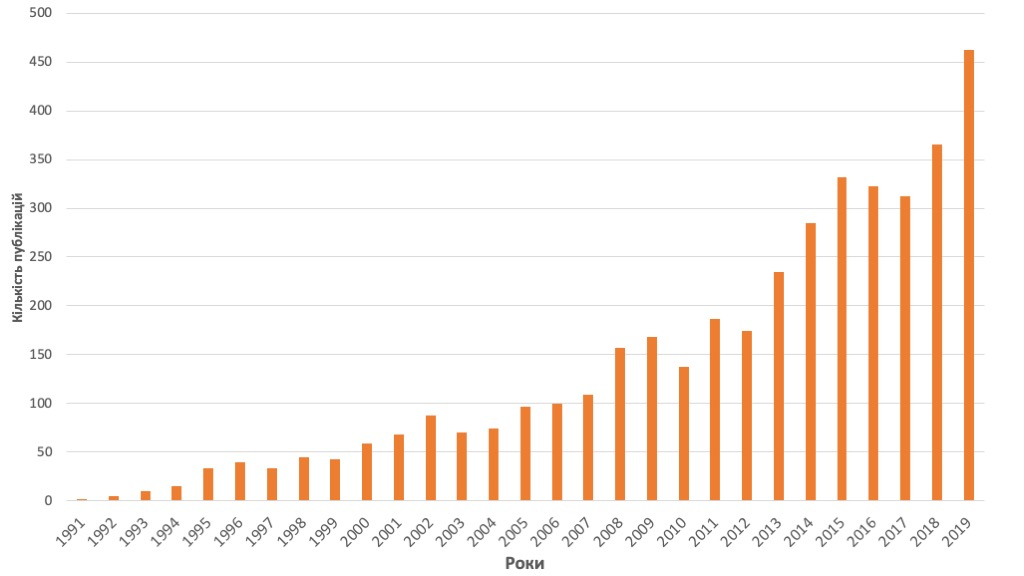
\includegraphics[width=0.9\textwidth]{Illustrations/Pic_01.jpg}
\label{fig:plot1}
\end{figure}

\subsubsection{Перша погоджувальна конференція} 

Перша погоджувальна конференція відбулась в Луізвілі в листопаді 2008 року за участі 45 міжнародних експертів з гепатобіліарної хірургії. \cite{Buell2009}. За результатами обговорення до  \acrshort{llr} були віднесені чисто лапароскопічні, хенд-асистовані резекції печінки (\acrshort{hals}) та гибридні резекції печінки (\acrshort{hlr}) при яких початкова диссекція проводиться в лапароскопічному варіанті а розсічення паренхіми через мінілапаротомію. 

Прийнятними для видалення за допомогою  \acrshort{llr} були визначені утворення, розміром менше 5 см, що розташовані в 2 - 6 сегментах печінки, а \acrshort{llls} було рекомендовано розглядати в якості стандартної практики. Також була показана принципова технічна можливість видалення новоутворень, локалізованих в будь яких сегментах печінки в лапароскопічному варіанті, проте обширні резекції печінки було рекомендовано зарезервувати за спеціалізованими гепатобіліарними центрами з великим досвідом як лапароскопічних втручаннь, так і резекційної хірургії печінки. 

Конверсію рекомендовано розглядати скоріше як необхідний крок для безпечного завершення складного втручання, ніж як ускладнення. Перед ургентною конверсією з приводу кровотечі хірург повинен докласти максимальних зусиль до зупинки кровотечі лапароскопічними методами. 

Вперше була показана можливість виконання донорського забору печінки при трансплантації від живого донора у дітей в лапароскопічному варіанті. Донорську \acrshort{llls} було оцінено, як експериментальну методику, що має великий потенціал але потребує детального вивчення. 

Вцілому консенсус визначив \acrshort{llr} як безпечну альтернативу традиційним резекціям та рекомендував методику до подальшого вивчення та більш широкого впровадження досвідченими гепатобіліарними хірургами.

\subsubsection{Друга погоджувальна конференція} 

На відміну від першої, друга погоджувальна конференція, яка відбулась в японському місті Моріока в жовтні 2014 році \cite{Kaneko2015}, була побудована за Цюріхсько-Датською моделлю, та включала в себе експертну панель з 43 досвідчених хірургів та 9 членів жюрі з 18 країн які оцінювали результати \acrshort{llr}. Для оцінки були запропоновані 17 запитаннь в категоріях переваги, ризики та технічні аспекти \acrshort{llr}, відповідаючи на які жюрі сформувало рекомендації. Доказова якість рекомендацій була оцінена за шкалою GRADE а ступінь розробки втручаннь за системою IDEAL \cite{Guyatt2008, McCulloch2009}. Для об'єму резекції було запропоноване класичне визначення: до малих резекцій (Minor resection) було віднести резекції 2 та меньше сегментів а до великих або обширних (Major resection) 3 та більше сегментів. Але зважаючи на те, що технічна складність \acrshort{llls} та правобічної задньої або передньої секцієектомії в лапароскопічному варіанті значно відрізняються, резекції, до складу яких входять сегменти 7 або 8 було віднесено до великих. 

За висновками експертного жюрі як малі так і великі \acrshort{llr} не гірші за відкриті в показниках операційної летальності, післяопераційних ускладненнь, чистоті резекційного краю, загальної виживаності та вартості операції та мають перевагу в більш короткому терміні перебування в стаціонарі, меншій крововтраті. Експерти погодились з тим, що результати лапароскопічних донорських заборів не відрізнялись від відкритих у високоспеціалізованих центрах. У якості додаткового висновку жюрі заключило, що великі \acrshort{llr} вимагають високого рівню хірургічних навичок та тривалої кривої навчання.

Основними досягненнями конференції було по-перше визнання того, що  \acrshort{llr} за більшістю показників не поступаються, а за окремими показниками перевершують відкриті втручання, а по-друге рекомендація використовувати малі \acrshort{llr} в якості стандарту надання допомоги.

\subsubsection{Створення клінічних рекомендацій} 
Подальший еспотенціальний ріст кількості \acrshort{llr} призвів до того, що в лютому 2017 року в Саузхемптоні була проведена третя погоджувальна конференція \cite{AbuHilal2017a} яка мала на меті створення загальноєвропейських клінічних рекомендацій. В процесі підготовки було залучено експертну панель з 11 досвідчених гепатобіліарних хірургів, частина з яких мала досвід лише відкритих резекцій печінки а частина як відкритих так і \acrshort{llr}. Після аналітичного обзору 647 джерел, відібраних за допомогою критеріїв включення експертами були сформовані рекомендації в п'яти ключових напрямках: покази, відбір пацієнтів, види втручаннь, технічні особливості та імплементація.

Згідно з цими рекомендаціями \acrshort{llr} показані для лікування метахронних колоректальних метастазів та гепатоцеллюлярної карциноми так як ассоційовані зі зниженням крововтрати, післяопераційного асциту, печінкової недостатності та терміну перебування в стаціонарі порівняно із відкритими втручаннями при порівняній тривалості операції, частоті R0 краю резекції та рівні рецидивів. Також \acrshort{llr} показані для лікування доброякісної вогнищевої патології завдяки суттєвому зниженню післяопераційних ускладненнь, больового синдрому та терміну перебування в стаціонарі, що підтверджено на великих серіях пацієнтів, у тому числі із великими резекціями. Донорські гепатектомії наразі не є добре стандартизованими процедурами та зарезервовані за високоспеціалізованими центрами.

Що до відбору пацієнтів, то \acrshort{llr} добре показали себе у хворих з вираженою коморбідністю та можуть бути рекомендовані для пацієнтів з ожирінням та пацієнтів старшого віку. Є данні, що свідчать про полегшення перебігу повторних (відкритих або лапароскопічних) резекцій печінки у пацієнтів, що перенесли \acrshort{llr} в якості первинної операції. Складні випадки з великими новоутвореннями (> 10 см) та близкістю до магістральних судин не є протипоказами до \acrshort{llr}, так як можуть бути виконані з аналогічною відкритим операціям  морбідністю.

Усі види \acrshort{llr}, як великі так і малі, асоційовані зі зменшенням інтраопераційної крововтрати, післяопераційних ускладненнь та терміну перебування в стаціонарі та аналогічними показниками онкологічної результативності порівняно з віткритими втручаннями. Великі втручання та втручання на задніх сегментах пов'язані із більшою складністю та тривалістю операції, проте в експертних центрах можуть бути досягнуті периопераційні результати аналогічні малим \acrshort{llr}.

Також в рекомнедаціях зазначено, що жодна з існуючих технік виконання \acrshort{llr} (\acrshort{hals}, \acrshort{hlr} або чисто лапароскопічна) не показала абсолютної переваги над іншими, проте вважається, що \acrshort{hals} та \acrshort{hlr} є перехідними до чисто лапароскопічної техніки. Те ж саме стосується й техніки транссекції паренхіми: краш-кламп, використання CUSA або інших хірургічних енергій визнано рівноцінними методами. Для диссекції портальних структур більшисть хірургів використовують ізольоване лігування, проте глісоновий підхід показав аналогічні результати. Для контролю кровотечі під час \acrshort{llr} рекомендовано використовувати лапароскопічний прийом Прінгла та анастезію з низьким центральним венозним тиском (\acrshort{cvp}). Факторами ризику конверсії на відкрите втручання є високий індекс маси тіла, розмір пухлини, локалізація ураження в постеролатеральних сегментах та цирроз. Перед виконанням ургентної конверсії рекомендовано досягти тимчасового гемостаза лапароскопічними методами.

Крива навчання малих \acrshort{llr} складає 60 випадків для хірурга, що має досвід відкритих резекцій печінки. Для великих \acrshort{llr} цей показник становить 55 операцій, при умові успішного проходження кривої для малих \acrshort{llr}. Впровадження \acrshort{llr} не повинно відбуватись в ізоляції від відкритої хірургії печінки. Для кожного спелізованого гепатобіліарного центру рекомендована наявність не менше двох хірургів, спеціалізованих на \acrshort{llr}.

Якщо послідовно проаналізувати висновки всіх погоджувальних конференцій стає зрозумілим, що методика \acrshort{llr} успішно пройшла крізь етапи розробки, первинної оцінки результатів та широкого впровадження базуючись на принципах доказової медицини. Чисельна кількість дослідженнь на великих групах пацієнтів \cite{Ciria2016b, Takahara2016, Berardi2017}, в тому числі два рандомізоаних клінічних дослідження \cite{Fretland2018b, Robles-Campos2019} свідчать про перевагу \acrshort{llr} над традиційними відкритими втручаннями в періопераційних показниках зі збереженням онкологічної ефективності. 

\section[Сучасні можливості]{Сучасні можливості лапароскопічної резекційної хірургії печінки}

\subsection{Анатомічні резекції печінки}
З моменту першої \acrshort{llr} можливості методу значно поширились за межі крайових резекцій новоутворень невеликого розміру. На данний момент показана доступність виконання в лапароскопічному варіанті абсолютно всіх видів анатомічних резекцій печінки при доброякісних та онкологічних пухлинах, включно навіть з операціями при хіларній холангіокарциномі. Найбільш часто вживані резекції, такі як \acrshort{llls}, лівобічна та правобічна гемігепатектомія та моносегментектомії є добре вивченими та стандартизованими процедурами, що дозволяє деяким спеціалізованим центрам \cite{Garbarino2019} виконувати до 80-90\% всіх резекцій печінки в лапароскопічному варіанті. Тож, в більшості випадків, вибір доступу визначається скоріше можливостями клініки ніж можливостями методики. 

За об'ємом розрізняють малі (Minor) та великі або обширні (Major) резекції. До малих резекцій відносять моно- та бісегментектомії антеролатеральних сегменітв та ліву латеральну секцієектомію. До великих або обширних анатомічних \acrshort{llr} відностяь резекції при яких виляляють три або більше розташованих поруч сегмента. Класичними представниками великих резекцій є лівобічна та правобічна гемігепатектомії.

\subsubsection{Лівобічна гемігепатектомія}

Лапароскопічна лівобічна гемігепатектомія (\acrshort{llhe}) показала себе як доступна, безпечна та ефективна процедура для пацієнтів, що мають новоутворення лівої долі печінки. В ретроспективному порівняльному аналізі 62 \acrshort{llhe} та 118 відкритих лівобічних гемігепатектомій у пацієнтів з гепатоцеллюлярною карциномою (\acrshort{hcc}), внутрішньопечінковою холангіокарциномою (\acrshort{ihcc}) та деякими доброякісними новоутвореннями показано перевагу лапароскопічних втручаннь за рахунок зменшення крововтрати, часу до відновлення харчування та частоти важких ускладненнь з порівняними показниками виживаності у онкологічних хворих \cite{Cho2018b}.   Міжнародне мультицентрове ретроспективне дослідження реузльтатів 82 \acrshort{llhe} \cite{Belli2013a} не виявило достовірної різниці кількості ускладненнь та періопераційних показників у порівнянні з 222 \acrshort{llls}, - процедурою, яка є визнаним "золотим стандартом". Не дивлячись на те, що \acrshort{llhe} є технічно складнішою за \acrshort{llls}, автори рекомендують її в якості стандартного методу лікування.

\subsubsection{Правобічна гемігепатектомія}

Лапароскопічна правобічна гемігепатектомія (\acrshort{lrhe}) є непростим втручанням, так як потребує повної мобілізації та маніпуляцій з об'ємною правою долею печінки, що потребує технічної майстерності від оперуючого хірурга. З моменту першого виконання Hüscher C. в 1995 році \cite{Huscher1997} техніка \acrshort{lrhe} вдосконалювалась та зазнавала постійних модифікацій \cite{Gayet2007, Dagher2008, Homma2019, Kim2017a}. В сучасному варіанті \acrshort{lrhe} є добре вивченою процедурою. Її онкологічна еффективність та рівень ускладнень у пацієнтів з ГЦК на фоні цирозу не відрізняється від традиційної відкритої правобічної гемігепатектомії за результатами корейського моноцентрового ретроспективного псевдорандомізованого дослідження \cite{Yoon2017b}. 

\subsubsection{Секцієектомії та центральні резекції}

Окрім \acrshort{llhe} та \acrshort{lrhe} обширні резекції включають в себе праву передню, праву задню та ліву медіальну секцієектомії, мезогепатектомію. Технічно такі операції вважаються складнішими за класичні гемігепатектомії, так як включають дві площини резекції, що знаходяться під кутом одна до одної. Не дивлячись на це, в серії дослідженнь показано, що такі втручання є безпечними та відтворюваними в експертних центрах \cite{Honda2014, Cheng2015, Kim2017, Siddiqi2018}. 

\subsubsection{Складні локалізації}

Постерокраніальні сегменти (Sg 7,8) та каудальна лобектомія певний час вважались недоступними для лапароскопічного доступу через високе незручне розтажування обмежене ребрами та куполом діафрагми, та анатомічну близкість до печінкових вен та нижньої порожнистої вени (\acrshort{ivc}). В 2014 роци Ban D. та співавтори розробили шкалу складності для \acrshort{llr}, де віднесли ізольовані лапароскопічні резекції Sg 7 та 8 до резекцій вищого ступеню складності, порівняно з резекціями інших анатомічних ділянок. Для полегшення доступу до постерокраніальних сегментів Ikeda T. була запропонована напівпронована позиція пацієнта та латеральний доступ до Sg 7-8 \cite{Ikeda2014}. Пізніше Honda G. та співавторами була опублікована методика анатомичної резекції Sg 7 з внутрішньопечінковим доступом до сегментарного  гліссону \cite{Okuda2017}, а Inoue Y. показано спосіб резекції Sg 6, 7 та 8 з латерального доступу з використанням трансторакальних троакарів \cite{Inoue2017}. Описаний досвід виконання атипових резекцій печінки трансторокальним доступом при вираженому злуковому процесі в черевній порожнині \cite{Kruger2014}. Суть методу полягає в доступі до Sg 8 з правої плевральної порожнини шляхом розсічення правого куполу діафрагми.

Складність каудальної лобектомії обумовлена тим, що перший сегмент розташований в позаду печінки і безпосередньо межує з \acrshort{ivc}, що робить його пряму візуалізацію неможливою та суттєво ускладнює хірургічний доступ. Окрім того каудальна доля має власні окремі печінкові вени, які дренуються в запечінковий сегмент \acrshort{ivc}, що підвищує ризик кровотечі під час його мобілізації і робить лапароскопічну каудальну лобектомію (\acrshort{lce}) складним втручанням. В літературі є обмежені згадки про досвід виконання \acrshort{lce} переважно у вигляді кейс-репортів та невеликих серій \cite{Machado2018, Cheung2016, Koh2017, Jin2018}. Найбільшою небезпекою, пов'язаною \acrshort{lce} вважають ризик розвитку масивної неконтрольованої кровотечі з передньої стінки \acrshort{ivc} або задньої стінки серединної печінкової вени (\acrshort{mhv}), при цьому загальна морбідність складає лише 6,6\% \cite{Araki2018}. Альтернативою до лапароскопічного підходу для виконання каудальної лобектомії може стати використання роботичних систем, які полегшують маніпуляції в обмеженому просторі \cite{Marino2018a}.

\subsection[Комплексні резекції]{Комплексні резекції у поєднанні з резекцією судин чи жовчних протоків, розширеною лімфодиссекцією}

У частини пацієнтів з поширеними формами злоякісних новоутвореннь печінки спостерігається інвазія в магістральні структури печінки - ворітну вену, печінкові вени або жовчні протоки. У більшості випадків таке ураження є протипоказом до хірургічного лікування з онкологічної точки зору, проте для певної категорії пацієнтів, що страждають на локалізовані форми метастазів колоректального раку в печінку (\acrshort{crlm}) або \acrshort{hcc} чи \acrshort{phcc} хірургічне лікування у вигляді комплексної резекції печінки в комбінації із судинною або біліарною резекцією може позитивно впливати на прогноз \cite{Kobayashi2015, Tardu2016, Procopio2020, Matsukuma2020}. В більшості випадків необхідність комплексної резекції є показом до відкритого втручання, проте деякими авторами описана можливість виконання таких втручань в лапароскопічному варіанті.

\subsubsection{Резекції судин}

Огляд літератури виявив невелику кількість випадків резекцій магістральних судин виконаних під час проведення лапароскопічної резекції печінки - 3 кейс-репорти та одне дослідження серії з 6 хворих. 
Так Nomi T. та співавт. повідомляють про успішний випадок крайової резекції \acrshort{ivc} під час проведення \acrshort{lrhe} переднім доступом у 58-річного пацієнта з приводу \acrshort{crlm} \cite{Nomi2015a}. Пізніше Vega E. та співавт. виконали \acrshort{lce} з частковою резекцією \acrshort{ivc} 54-річному пацієнту, що страждав \acrshort{hcc} на фоні цирозу \cite{Vega2020}. 
Lopez-Ben та співавтори показали двохетапний лапароскопічний підхід при видаленні білобарних \acrshort{crlm} 66-річному пацієнту. Першим етапом була виконана лапароскопічна правобічна задня секцієектомія (\acrshort{lrps}) з резекцією та реконструкцією шляхом формування судинного анастомозу правої печінкової вени (\acrshort{rhv}). Під час другого етапу була виконана \acrshort{llhe}. Автори повідомляють про хороший онкологічний ефект операції та відсутність рецидивів під час огляду через 2 роки після втручання \cite{Lopez-Ben2020}.
Єдине дослідження серії випадків судинних резекцій під час проведення \acrshort{llr} належить Morise Z. та співавторам \cite{Morise2015a}. Автори заявляють про досвід 98 \acrshort{llr} з приводу \acrshort{hcc} на фоні цирозу, 6 з яких було виконано резекцію стовбура однієї з магістральних печінкових вен за допомогою лінійного степлера.
Не дивлячись на достатньо поширене застосування резекції та реконструкції стовбура ворітної вени під час виконання лапароскопічної панкреатодуоденальної резекції \cite{Kendrick2011, Garbarino2018, Wei2019} нами не було знайдено джерел, що описують застосування портопластики під час проведення \acrshort{llr}, що скоріше за все пов'язано із її технічною складністю та обмеженістю показів. 

\subsubsection{Біліарні реконструкції}

Резекція позапечінкових жовчних шляхів є обов'язковим етапом радикальних резекцій печінки з приводу \acrshort{phcc} а також може бути застосована при пухлинній інвазії іншими пухлинами. В лапароскопічному варіанті, як самостійне втручання гепатикоєюностомія широко використовується при кистах та стриктурах холедоха, як паліативне втручання, а також як частина панкреатодуоденальної резекції при пухлинах голівки підшлункової залози. Згідно доступних даних \acrshort{llr} з приводу  \acrshort{phcc} все ще є новітньою процедурою на стадії вивчення, тому досвід виконання таких операцій обмежений кейс-репортами \cite{Lin2014, Machado2014} або невеликими серіями \cite{Ratti2020}. Таким чином в експертних центрах гепатикоєюностомія є технічно доступним етапом при виконанні \acrshort{llr}, а впровадження роботичної хірургії дає надію на її більш широке застосування \cite{Machado2019, Giulianotti2010}

\subsubsection{Розширена лімфаденектомія}

Лімфодиссекція є стандартизованим етапом багатьох лапароскопічних операцій з приводу онкопатології, зокрема в мініінвазивній гінекології та хірургії шлунково-кишкового тракту \cite{Eshuis2018, Jung2019}. В резекційній хірургії печінки лімфодиссекція показана при наявності локального позапечінкового ураження лімфовузлів наприклад при \acrshort{crlm}. Не дивлячись на те, що  онкологічна ефективність привентивної лімфаденектомії при \acrshort{llr} з приводу \acrshort{ihcc} остаточно не доведена \cite{Weber2015, Zhou2019a}, багато хірургів рекомендують її рутинне виконання з метою адекватного стадіювання пухлини та визначення прогнозу \cite{Waisberg2018, Ratti2020a}.

Більшість данних про лімфаденектомію як етап \acrshort{llr} представлені у вигляді кейс-репортів та серій випадків. Їх узагальнення  наведено Levi Sandri G.B. та співавторами в оглядовій статті, на основі чого автори роблять висновог про безпечність та доступність лапароскопічного підходу \cite{Colasanti2017}. Також є результати моноцентрового псевдорандомізованого дослідження в якому Ratti F. зі співавторами порівнюють 20 пацієнтів, що перенесли \acrshort{llr} з приводу \acrshort{ihcc} із 60 аналогічними відкритими операціями. За отриманими результатами \acrshort{llr}, серед яких 85\% великих резекцій, були не гіршими від відкритих втручаннь за показниками морбідності та безрецидивної виживаності, а також були асоційовані із меншою крововтратою та більшою кількістю видалених лімфовузлів \cite{Ratti2016a}. 

\subsection{Технологія ALPPS} 

В перше технологія Associating Liver Partition and Portal vein Ligation for Staged hepatectomy(\acrshort{alpps}) була запропонована в 2011  Lang H.  \cite{Baumgart2011} в якості альтернативи звичайній двоетапній резекції печінки з лігуванням ворітної вени. Суть нововведення полягала в тому, що на першому етапі проводять санацію планованого печінкового залишку, лігування ворітного притоку  частини печінки, що видаляють та транссекція паренхіми. При цьому за рахунок потужного викиду прозапальних факторів протягом 7-14 днів відбувається швидкий приріст об'єму планованого печінкового залишку, після чого виконують другий етап, під час якого видаляють депорталізовану на першому етапі частину печінки. 

Методика привернула увагу науковців та отримала багатьох прихильників серед гепатобіліарних хірургів, як метод, що дозволяє значно розширити межі резектабельності у пацієнтів з обширними формами \acrshort{crlm} та інших пухлин завдяки інтенсивній регенерації печінкового залишку. Критики методики зазначали, що окрім переваг вона має певні недоліки, а саме високу частоту післяопераційних ускладненнь та ризики прогрессії пухлини між першим та другим етапами. 

Для подолання цих недоліків Brustia R. та співавторами було запропоновано виконувати втручання в лапароскопічному варіанті \cite{Brustia2013}. Наразі загальна кількість таких операцій не велика, що може бути пов'язано з тим, що відкрита  \acrshort{alpps} є відносно новим та методом, який досі знаходиться на етапі дослідження \cite{Melandro2019}.Так, Michal K. та співавтори \cite{Michal2020} за результатами метааналізу 23 джерел порівняли 46 мініінвазивних та 1088 відкритих \acrshort{alpps}, та дійшли до висновку, що лапароскопічні та роботичні втручання дозволяють знизити частоту ускладненнь порівняно з відкритими втручаннями та отримати більший ступінь гіпертрофії порівняно з емболізацією ворітної вени. До недоліків мініінвазивного підходу автори відносять ризик виявлення лише частини наявних вогнищ в наслідок обмеженої здатності до пальпації та складність імплементації такої процедури. 

\subsection{Лапароскопічна донорська резекція печінки} 

Трансплантація печінки від живого донора стала радикальним методом лікування дифузних захворюваннь та деяких пухлин печінки в умовах відсутності або обмеженої кількості трупних донорів. На відміну від резекцій з приводу новоутвореннь, під час виконання донорської резекції печінки перед хірургом стоять два завдання: по-перше це забезпечення безпеки та збереження здоров'я донора, по-друге забір реплантабельного та функціонального трансплантату з достатньою довжиною та придатним для пластики краєм ворітної та печінкових вен, печінкової артерії та жовчних протоків. 

Для зменшення ризику ускладненнь та раннього повернення працездатності донору в 2002 р. Cherqui D. та співавторами було запропоновано виконання донорського забору лівої латеральної секції в лапароскопічному варіанті при трансплантації дітям \cite{Cherqui2002a}. Пізніше техніка операції була адаптована та імплементована деякими центрами. Так наприклад Kim K-H. та свпіватори повідомляють про переваги лапароскопічного донорського забору лівої латеральної секції у вигляді зменшення терміну госпіталізації та пришвидшення реабілітації донора за результатами порівняння 11 таких втручаннь із 11 відкритими донорськими резекціями \cite{Kim2011}. 

Технічно більш складна донорська правобічна гемігепатектомія певний час залишалась недоступною для чисто лапароскопічного доступу. Запропоновані \acrshort{hals} та \acrshort{hlr} підходи не набули широкого розповсюдження \cite{Koffron2006, Thenappan2011, Lin2013}. Лише в 2013 р. Soubrane O. та співавторами була показана можливість донорського забору трансплантату правої долі печінки в чисто лапаропскопічному доступі \cite{Soubrane2013}. 

На теперішній момент лапароскопічний донорська гепатектомія активно застосовується більшістю великих спеціалізованих трансплантаційних центрів. Доступні результати псевдорандомізованих порівняльних дослідженнь, які демонструють переваги лапароскопічних донорських заборів над відкритими  аналогічні звичайним \acrshort{llr} при вогнищевій патології \cite{Broering2018, Park2019a}. Також показано безпеку лапароскопічного забору для реципієтнів \cite{Kwon2018a}. Йде дискуссія про стандартизацію та повсюдне впровадження методу \cite{Au2018, Samstein2018}


Таким чином за свою майже 30-річну історію \acrshort{llr} вийшла далеко за межі крайових та атипових резекцій антеролатеральних сегментів та впевнено конкурує з відкритими втручаннями у всіх галузях гепатобіліарної хірургії. 

\printbibliography[heading=subbibliography]

\end{refsection}  
\chapter[Планування та підготовка]{Планування та підготовка до лапароскопічних резекцій печінки}
\begin{refsection}

\section{Покази до виконання лапароскопічних резекцій печінки}

Технічні можливості лапароскопічної хірургії постійно зростають а хірургічна техніка вдосконалюється завдяки чому більшість втручаннь, що раніше виконувались лише у відкритому доступі зараз можлива і в лапароскопічному варіанті. Враховуючи сучасні досягнення покази до \acrshort{llr} практично не відрізняються від показів до \acrshort{olr} - лапароскопічний досуп не обмежує хірургічні можливості, проте додає певні властиві саме йому особливості. 

Серед показів до резекції печінки розрізняють злоякісну та доброякісну патологію. Серед онкопатології, на долю якої приходиться 60-80\% резекцій  найбільш частими показами до хірургічного лікування є первинні пухлини печінки та жовчних шляхів, а саме гепатоцелюлярна карцинома (\acrshort{hcc}), внутрішньопечінкова (або масформуюча) холангіокарцинома (\acrshort{ihcc}), перихіларна холангіокарцинома (\acrshort{phcc}), рак жовчного міхура (\acrshort{gbc}) та метастази колоректального раку в печінку \acrshort{crlm}. 

В цьому розділі ми зосередимось на тих видах хірургічної патології печінки, при яких застосування мініінвазивного підходу дає можливість отримати найкращі результати. 

\subsection{Гепатоцеллюларна карцинома}.

Гепатоцеллюлярна карцинома (\acrshort{hcc}) є п'ятою за частотою серед причин летальності від онкологічних захворюваннь. Причиною цього є  виявлення пізніх стадій захворювання через його асимптоматичний перебіг. Поширені форми \acrshort{hcc} характеризуються судинною інвазією, яка значно утруднює їх хірургічне лікування, а також наявністю у більшості хворих супутнього хронічного захворювання печінки та цирозу які суттєво погіршують печінкову функцію. Окрім того \acrshort{hcc} є хіміорезистентною пухлиною, що робить системну хіміотерапію не ефективною.

Сучасний підхід до лікування \acrshort{hcc} базується на виборі методу лікування в залежності від стадії пухлини. Найбільш часто вживаною системою стаціювання \acrshort{hcc} є барселонська (\acrfull{bclc}, \acrshort{bclc}) \cite{Llovet2003}. Згідно \acrshort{bclc} хірургічне лікування показано на ранній та дуже ранній стадіях \acrshort{hcc}, коли пухлина представлена солітарними резектабельними вузлами, а можливми опціями лікування є етанолова або радіочастотна абляція, відкрита або лапароскопічна резекція та трансплантація печінки. 

При дуже ранній стадії \acrshort{hcc} за \acrshort{bclc} з розміром вогнища до 2 см найбільш ефективні етанолова та радіочастотна абляція  \cite{Cucchetti2013}. Пацієнтам з \acrshort{hcc} в межах міланських критеріїв та декомпенсованим цирозом печінки оптимальним методом лікування є трансплантація печінки \cite{Colombo2016}. Для всіх інших пацієнтів з резектабельними формами \acrshort{hcc} методом першого вибору є резекція печінки \cite{Heimbach2018, Kudo2011}. 

\subsubsection{Анатомічна та неанатомічна резекція} 
\acrshort{hcc} --- агресивна високоінвазивна пухлина, яка має тенденцію до ураження малих та великих внутрішньопечінкових судин, периваскулярних компартментів та жовчних шляхів. Портальні тромби спричинені судинною інвазією можуть викликати кавернозну трансформацію та перивенозну колатеральну сітку. Мікросудинна інвазія це типова особливість \acrshort{hcc}, характерна переважно менш діфференційованим пухлинам, яка підтверджує агрессивну біологію пухлини. Незалежними предикторами мікроваскулярної інвазії є розмір пухлини більший 5 см., та менший ступінь дифференціації \cite{Zimmermann2017}. Інвазія в дрібні внутрішньопечінкові гілки ворітної вени може приводити до локального ретропортального кровотоку та периферійного внутрішньопечінкового розповсюдження у вигляді числених метастатичних вузлів по ходу судин в межах портального судинного басейну локальної анатомічної ділянки \cite{Kim2008}. 

Враховуючи схильність \acrshort{hcc} до локального метастазування в межах анатомічних ділянок методом вибору хірургічного лікування є анатомічна резекція печінки (\acrshort{alr}). На відміну від неанатомічної резекції печінки (\acrshort{non-alr}) \acrshort{alr} включає в себе ідентифікацію судинного бассейну анатомічної ділянки, що містить пухлину та видалення всієї її паренхіми. Онкологічні переваги \acrshort{alr} підтверждують більшість дослідженнь, так Makuuchi M. та співавтори \cite{Shindoh2016} в дослідженні 209 пацієнтів з цирозом класу А за Чайлдом та \acrshort{hcc} розміром $\leq$ 5 см, що були резектабельні як за допомогою \acrshort{alr} так і \acrshort{non-alr} показали перевагу \acrshort{alr} завдяки меншому ризику локальних рецидивів та більшій тривалості життя. Автори метааналізу \cite{Moris2018} 43 досліджень стверджують, що у 6839 пацієнтів яким була виконана \acrshort{alr} в порівнянні з 5590 пацієнтами з \acrshort{non-alr} були кращі загальна та безрецидивна виживаність та морбідність та рання післяопераційна летальність.

До переваг \acrshort{alr} відносять кращий онкологічний ефект, а до недоліків - вищий порівняно з \acrshort{non-alr} ризик післяопераційного порушення печінкової функції, пов'язаний з більшим об'ємом резекції, що особливо важливо для пацієнтів із цирозом печінки. Враховуючи це необхідний ретельний відбір пацієнтів для резекції печінки з приводу \acrshort{hcc}, що базується на оцінці рівню печінкової недостатності, ступеню портальної гіпертензії та загального статусу пацієнта. Американські клінічні настанови National Comprehensive Cancer Network (\acrshort{NCCN}) в якості кандидатів для резекції печінки пропонують пацієнтів з компенсованою печінковою функцією, солітарним вогнищем без макросудинної інвазії та майбутнім печінковим залишком (\acrshort{flr}) $\geq$ 20\% для здорової паренхіми та $\geq$ 30-40\% з адекватним кровопостачанням та жовчевідтоком. В клінічних настановах Європейської ассоціації вивчення хвороб печінки по лікуванню \acrshort{hcc} \cite{Galle2018a} для пацієнтів з цирозом печінки запропоновано спрощений алгорим визначення ризику \acrshort{alr}, що базується на об'ємі резекції, супеню портальної гіпертензії та печінкової недостатності. 

\subsubsection{Лапароскопічна та відкрита резекція печінки при \acrshort{hcc}} 
Окрім віддалених результатів на ефективність лікування впливає післяопераційна морбідність. Першим з двох основних факторів, які впливають на післяопераційні результати під час резекції печінки з приводу \acrshort{hcc} є крововтрата. Вищий об'єм крововтрати та замісної трансфузії препаратів крові асоційований з вищою з частотою післяопераційних ускладненнь та меншою віддаленою виживаністю \cite{DeBoer2007, Romano2012}. Крововтрата викликає імунодепрессію що сприяє розвитку хірургічних інфекцій, сепсису і збільшення ризику рецидиву в подальшому. Другим фактором є післяопераційна асцитопродукція у пацієнтів з цирозом печінки, яка є грізним ускладненням, що може призводити до великих втрат білка та рідини (до 5 літрів на добу), нагноєння післяопераційної рани та погіршання печінкової функції \cite{Ishii2014}. Окрім збільшення резистивності портального русла через його зменшення внаслідок резекції печінки та набряку печінкового залишку, механізм виникнення асцитопродукції пов'язують з декомпенсацією портальної гіпертензії внаслідок переривання портосистемної колатералізації під час лапаротомії \cite{Kanazawa2013}. 

Згідно існуючих даних, лапароскопічний підхід ефективно знижує ризики обох цих ускладненнь. За рахунок більш прецизійної техніки та позитивного тиску карбоксиперитонеуму \acrshort{llr} асоційовані з меншою інтраопераційною крововтратою, а збереження цілісності колатералей передньої черевної стінки дозволяє знизити частоту та інтенсивність післяопераційної асцитопродукції \cite{Truant2011}. Також \acrshort{llr} зменшують і загальну післяопераційну морбідніть у пацієнтів з \acrshort{hcc} на фоні цирозу при вираженій портальній гіпертензії та тромбоцитопенії < 100,000/мл про що свідчать результати міжнародного мультицентрового порівняльного псевдорандомізованого дослідження результатів лікування 1974 пацієнтів \cite{Ruzzenente2020}.

\emph{Враховуючи наведене вище оптимальними показами до \acrshort{llr} при \acrshort{hcc} є резектабельні форми пухлини всіх локалізацій без ураження магістральних судин або жовчних протоків на фоні здорової паренхіми або компенсованого цирозу печінки при відсутності показів до трансплантації печінки.}

\subsection{Рак біліарного тракту}

Рак біліарного тракту (\acrshort{btc}) - гетерогенна група захворюваннь до якої відносять внутрішньопечінкову (або масформуючу) холангіокарциному (\acrshort{ihcc}), перихіларну холангіокарциному (\acrshort{phcc}), рак жовчного міхура (\acrshort{gbc}) покази до лікування яких за допомогою \acrshort{llr} будуть розглянуті нижче, та рак дистального відділу холедоха і ампулярний рак, які не відносяться до теми цієї книги. 

\subsubsection{Внутрішньопечінкова масформуюча холангіокарцинома}

\acrshort{ihcc} є другою за частотою формою первинного рака печінки з високим потенціалом диссемінації та рецидивів, що походить із клітин проксимальних гілок жовчних протоків, на долю якої припадає до 40\% первинних пухлин печінки. Резекція печінки є єдиним потенційно радикальним методом та застосовується в якості першого етапу лікування \acrshort{ihcc}. Медіана виживаності пацієнтів після радикальної резекції складає 27 - 36 міс \cite{Buettner2017}. Не дивлячись на те, що вплив лімфаденектомії на виживаність при \acrshort{ihcc} остаточно не доказано рекомнедується її рутинне виконання з метою стадіювання процесу та вибору подальшого лікування. При досягненні R0 резекцийного краю необхідна системна адьювантна хіміотерапія, яка може бути доповнена хеморадіаційними методами в разі R1 резекції або позитивних лімфовузлів. При досягненні R2 резекцийного краю із макроскопічними залишками пухлини подальше лікування пацієнта необхідно проводити згідно рекомендацій до лікування нерезектабельних форм \acrshort{ihcc}. 

Резекція печінки при \acrshort{ihcc} є комплексною процедурою, технічна складність якої посилюється лімфаденектомією та можливою резекцією позапечінкових жовчних шляхів. Не дивлячись на те, що Саузґемптонські рекомендації не визначають однозначно місце \acrshort{llr} в лікуванні \acrshort{ihcc} через обмежену кількість накопиченого досвіду внаслідок низької частоти резектабельних форм, існує кілька порівняльних дослідженнь, що свідчать на користь лапароскопічного доступу. Так, група південнокорейських авторів на основі порівняння результатів 14 \acrshort{llr} з результатами 23 \acrshort{olr} у пацієнтів з \acrshort{ihcc} зазначає, що при порівняних онкологічних результатах пацієнти, що перенесли \acrshort{llr} мали меншу крововтрату та кращі ранні післяопераційні показники \cite{Lee2016a}. Характерною особливістю дослідження є те, що в нього включені лише невеликі пухлини, розміром $\leq$ 5 см. Ці данні також підтверджує двоцентрове псевдорандомізоване дослідження групи італійських та англійських вчених, в якому на основі вивчення результатів 208 \acrshort{llr} та \acrshort{olr} автори визначають \acrshort{llr} у відібраних пацієнтів  з \acrshort{ihcc}, як доступну та онкологічно ефективну процедуру, асоційовану з меншим ризиком післяопераційних ускладненнь \cite{Ratti2020}.


\subsubsection{Перихіларна холангіокарцинома}

На відміну від інших видів \acrshort{btc}, \acrshort{phcc}, це захворювання при якому показана можливість 10-річної виживаності після хірургічного лікування на рівні 14\% при адекватному відборі пацієнтв \cite{Juntermanns2019}. Через свої біологічні особливості \acrshort{phcc} має схильність до підслизового інфільтративного росту \cite{Sakamoto1998}, що обумовлює поширення пухлини за межі макроскопічно ураження, а також до інвазії магістральних судин ще до клінічної маніфестації у вигляді механічної жовтяниці \cite{Shimada2003}. Пухлина частіше розповсюджується лімфогенним та периневральним, ніж гематогенним шляхом \cite{Zimmermann2017}. Ці морфологічні особливості визначають агресивну хірургічну тактику та об'єм  втручання при \acrshort{phcc}, яке включає резекцію печінки відповідно рівню ураження із тотальною каудальною лобектомією, резекцію позапечінкових жовчних шляхів та розширену лімфаденектомію. За необхідості втручання може бути доповнене резекцією ворітної вени та печінкової артерії при їх пухлинній інвазії а також панкреатодуоденальною резекцією при інвазії дистального края холедоха \cite{Mizuno2019}. 

Через обширність та складність втручання в літературі доступні обмежені данні про мініінвазивне оперативне лікування \acrshort{phcc}. За данними огляду літератури та метааналізу групою авторів з нідерландів у 15 джерелах загалом виявлено 142 випадки виконання радикального мініінвазивного втручання з приводу \acrshort{phcc}, з яких 82 були \acrshort{llr} і 59 робот-асистованими резекціями \cite{Mizuno2019}. Дослідження виявило, що мініінвазивний підхід дає можливість отримати післяопераційну морбідність на рівні 24\% та летальність на рівні 3\%, що порівняно з результатами відкритих резекцій, та досягнути R0 резекції у 80\%. Не зважаючи на отримані оптимістичні результати, автори досить стримані у висновках, що обумовлено недостатньою кількістю накопиченого в світі досвіду та можливістю систематичної похибки через оцінку невеликих ретельно відібраних серій випадків. 

\subsubsection{Рак жовчного міхура}

\acrshort{gbc} є найбільш агресивною формою \acrshort{btc} з медіаною виживаності без лікування 6-10 місяців \cite{Lindner2018}, що пов'язано із асимптоматичним перебігом та пізнім виявленням. Радикальне хірургічна резекція може покращити результати виживаності із досягненням медіани 32 місяців. Сучасна тактика вибору об'єму хірургічного лікування \acrshort{gbc}, зазначена в рекомендаціях \acrshort{NCCN} з лікування гепатобіліарного раку, базується на стадії захворювання та обставинах його виявлення. При аксідентальному виявленні резектабельної ранньої форми \acrshort{gbc} під час холецистектомії остання доповнюється резекцією ложа жовчного міхура печінки. При виявленні пухлини під час планової проводки гістологічного препарату на стадії T1a (без інвазії підслизового шару) рекомендовано подальше спостереження, а на стадії T1b та вище, то в залежності від об'єму інвазії в паренхіму рекомендовано виконання другим етапом резекції Sg 4a-5 печінки або правобічної трисекцієектомії з лімфаденектомією. Резекція позапечінкових жовчних шляхів виконується в залежності від наявності ураження дистального краю міхурової протоки. Виконання резекції позапечінкових жовчних шляхів з метою розширення об'єму лімфаденектомії не є виправданим.  При доопераційному виявленні \acrshort{gbc} план втручання обирається в залежності від об'єму ураження.

В рекомендаціях по лікуванню \acrshort{btc} японської спілки гепатобіліарних хірургів 2015 року зазначається, що \acrshort{gbc} є протипоказом до лапароскопічної холецистектомії у зв'язку із високим ризиком диссемінації та портових метастазів \cite{Miyazaki2015}. Проте в більш пізньому міжнародному експертному консенсусі з лапароскопічної хірургії \acrshort{gbc} 2019 року наголошується, що лапароскопічний доступ не асоційований із погіршенням виживаності при ранніх стадіях \acrshort{gbc} (Т1,Т2) не ассоційованого із гострим холециститом, якщо виконується радикальна резекція, а доведеною причиною диссемінації є пошкодження цілісності стінки жовчного міхура та видалення макропрепарату без використання контейнера. У висновках консенсуса зазначається, що незважаючи на те, що \acrshort{llr} при \acrshort{gbc} є втручанням на ранніх стадіях вивчення, вона не погіршує прогноз, а у ретельно відібраних пацієнтів може покращувати результат операції. 


\emph{Таким чином, на теперішній момент \acrshort{llr} при всіх видах \acrshort{btc} є новою перспективною методикою на етапі вивчення, тому виконання цих операцій обмежено спеціалізованими центрами гепатобіліарної хірургії з великим досвідом мініінвазивних втручаннь.}

\subsection{Метастатичні ураження печінки}

\subsubsection{Метастатичний колоректальний рак}

\subsubsection{Метастатичний рак печінки не колоректального походження}


\subsection{Доброякісна патологія печінки}

\subsubsection{Аденоми печінки}

\subsubsection{Кистозні ураження печінки}

\subsubsection{Внутрішньопечінковий холелітіаз}


%%%%%%%%%%%%%%%%%%%%%%%%%%%%%%%%%%%%%%%%%%%%%%%%%%%%%%%%
%%%%%%%%%%%%%%%%%%%%%%%%%%%%%%%%%%%%%%%%%%%%%%%%%%%%%%%%
%%%%%%%%%%%%%%%%%%%%%%%%%%%%%%%%%%%%%%%%%%%%%%%%%%%%%%%%




\section{Лапароскопічний погляд на хірургічну анатомію печінки}

\subsection{Сучасні принципи хірургічної анатомії печінки}

\subsection{Портальна сегментація печінки}

\subsection{Капсула Лаенека та «вхідні ворота»}

\subsection{Печінкові вени як направляючі для плошини резекції}

\subsection{Анатомія першого сегменту печінки}


\section{Технічне забезпечення лапароскопічних резекцій печінки}

\subsection{Вимоги до лапароскопічної стійки}

\subsection{Інструменти доступу та видалення препарату}

\subsection{Базові інструменти}

\subsection{Зшиваючі аппарати}

\subsection{Хірургічні енергії}

\subsection{Спеціалізоване обладнання}


\printbibliography [heading=subbibliography]
\end{refsection}
\chapter{Техніка окремих видів лапароскопічних резекцій печінки} 

\begin{refsection}

\section{Атипова резекція печінки}

\section{Лівобічна латеральна секцієектомія}

\section{Моносегментектомія антеролатеральних сегментів}

\section{Бісегментектомія антеролатеральних сегментів}

\section{Лівобічна гемігепатектомія}

\section{Правобічна гемігепатектомія}

\section{Правобічна задня секцієектомія}



\printbibliography [heading=subbibliography]
\end{refsection}
\chapter{Техніка окремих типів втручаннь}
\begin{refsection}
\section{Атипова резекція печінки}

\section{Лівобічна латеральна секцієектомія}

\section{Моносегментектомія антеролатеральних сегментів}

\section{Бісегментектомія антеролатеральних сегментів}

\section{Лівобічна гемігепатектомія}

\section{Правобічна гемігепатектомія}

\section{Правобічна задня секцієектомія}

Текст
\printbibliography [heading=subbibliography]
\end{refsection} 
%\chapter{Шаблон глави}
\begin{refsection}
\begin{chapquote}{Author's name, \textit{Source of this quote}}
``This is a quote and I don't know who said this.''
\end{chapquote}

\section{Заголовок секції}
Lorem ipsum dolor sit amet, consectetur adipisicing elit, sed do eiusmod tempor incididunt ut labore et dolore magna aliqua. Ut enim ad minim veniam, quis nostrud exercitation ullamco laboris nisi ut aliquip ex ea commodo consequat. \\ Duis aute irure dolor in reprehenderit in voluptate velit esse cillum dolore eu fugiat nulla pariatur. Excepteur sint occaecat cupidatat non proident, sunt in culpa qui officia deserunt mollit anim id est laborum. \\ Lorem ipsum list:

1. Lorem ipsum dolor sit amet, consectetur adipiscing elit.

2. Duis ac mi magna, a consectetur elit.

3. Curabitur posuere erat \emph{dignissim ligula euismod} ut euismod nisi.

4. Fusce vulputate facilisis neque, et ornare mauris mattis vel.

5. Mauris sit amet nulla mi, vitae rutrum ante.

6. Maecenas quis nulla risus, vel tincidunt ligula.

7. Nullam ac enim neque, non \emph{dapibus} mauris.

8. Integer volutpat leo a orci suscipit eget rhoncus urna eleifend.

\noindent Цей параграф починається без відступу. Lorem ipsum dolor sit amet, consectetur adipiscing elit. Duis risus ante, auctor et pulvinar non, posuere ac lacus. Praesent egestas nisi id metus rhoncus ac lobortis sem hendrerit. Etiam et sapien eget lectus interdum posuere sit amet ac urna\footnote{Lorem ipsum dolor sit amet, consectetur adipiscing elit. Duis risus ante, auctor et pulvinar non, posuere ac lacus.}:

\subsection{Субсекція}
Lorem ipsum dolor sit amet, consectetur adipiscing elit. Duis risus ante, auctor et pulvinar non, posuere ac lacus. Praesent egestas nisi id metus rhoncus ac lobortis sem hendrerit. Etiam et sapien eget lectus interdum posuere sit amet ac urna. Aliquam pellentesque imperdiet erat, eget consectetur felis malesuada quis. Pellentesque sollicitudin, odio sed dapibus eleifend, magna sem luctus turpis, id aliquam felis dolor eu diam. Etiam ullamcorper, nunc a accumsan adipiscing, turpis odio bibendum erat, id convallis magna eros nec metus. Sed vel ligula justo, sit amet vestibulum dolor. Sed vitae augue sit amet magna ullamcorper suscipit. Quisque dictum ipsum a sapien egestas facilisis.

Цей параграф починається з червоної строки. Lorem ipsum dolor sit amet, consectetur adipiscing elit. Duis risus ante, auctor et pulvinar non, posuere ac lacus. Praesent egestas nisi id metus rhoncus ac lobortis sem hendrerit. Etiam et sapien eget lectus interdum posuere sit amet ac urna.

\subsection{Ще одна субсекція}
Lorem ipsum dolor sit amet, consectetur adipiscing elit. Duis risus ante, auctor et pulvinar non, posuere ac lacus. Praesent egestas nisi id metus rhoncus ac lobortis sem hendrerit. Etiam et sapien eget lectus interdum posuere sit amet ac urna. Aliquam pellentesque imperdiet erat, eget consectetur felis malesuada quis. Pellentesque sollicitudin, odio sed dapibus eleifend, magna sem luctus turpis, id aliquam felis dolor eu diam.

\subsection{І ще одна субсекція}
Lorem ipsum dolor sit amet, consectetur adipiscing elit. Duis risus ante, auctor et pulvinar non, posuere ac lacus. Praesent egestas nisi id metus rhoncus ac lobortis sem hendrerit. Etiam et sapien eget lectus interdum posuere sit amet ac urna. Aliquam pellentesque imperdiet\footnote{\url{www.example.com}} erat, eget consectetur felis malesuada quis. Pellentesque sollicitudin, odio sed dapibus eleifend, magna sem luctus turpis, id aliquam felis dolor eu diam. Etiam ullamcorper, nunc a accumsan adipiscing, turpis odio bibendum erat, id convallis magna eros nec metus. Sed vel ligula justo, sit amet vestibulum dolor. Sed vitae augue sit amet magna ullamcorper suscipit. Quisque dictum ipsum a sapien egestas facilisis.

In hac habitasse platea dictumst. Nullam turpis erat, porttitor ut pretium ac, condimentum sed dui. Praesent arcu elit, tristique sit amet viverra at, auctor quis tortor. Etiam eleifend posuere aliquam. Donec sed mattis sapien. Aenean urna arcu, suscipit at rutrum ac, adipiscing ac felis. Class aptent taciti sociosqu ad litora torquent per conubia nostra, per inceptos himenaeos. Praesent condimentum felis a ipsum ullamcorper semper. Vivamus eu odio sem, dictum luctus nunc. Etiam tincidunt venenatis dolor non pellentesque.

\subsection{Lorem ipsum dolor sit amet, auctor et pulvinar non}
Lorem ipsum dolor sit amet, consectetur adipiscing elit. Duis risus ante, auctor et pulvinar non, posuere ac lacus. Praesent egestas nisi id metus rhoncus ac lobortis sem hendrerit. Etiam et sapien eget lectus interdum posuere sit amet ac urna. Aliquam pellentesque imperdiet erat, eget consectetur felis malesuada quis. Pellentesque sollicitudin, odio sed dapibus eleifend, magna sem luctus turpis, id aliquam felis dolor eu diam. Etiam ullamcorper, nunc a accumsan adipiscing, turpis odio bibendum erat, id convallis magna eros nec metus. Sed vel ligula justo, sit amet vestibulum dolor. Sed vitae augue sit amet magna ullamcorper suscipit. Quisque dictum ipsum a sapien egestas facilisis.

In hac habitasse platea dictumst. Nullam turpis erat, porttitor ut pretium ac, condimentum sed dui. Praesent arcu elit, tristique sit amet viverra at, auctor quis tortor. Etiam eleifend posuere aliquam. Donec sed mattis sapien. Aenean urna arcu, suscipit at rutrum ac, adipiscing ac felis. Class aptent taciti sociosqu ad litora torquent per conubia nostra, per inceptos himenaeos. Praesent condimentum felis a ipsum ullamcorper semper. Vivamus eu odio sem, dictum luctus nunc. Etiam tincidunt venenatis dolor non pellentesque. 


\section{Another section heading}
Lorem ipsum dolor sit amet, consectetur adipisicing elit, sed do eiusmod tempor incididunt ut labore et dolore magna aliqua. Ut enim ad minim veniam, quis nostrud exercitation ullamco laboris nisi ut aliquip ex ea commodo consequat.

%%%%%%%%%%%%%%%%%%%%%%%%%%%%%%%%%%%%%%%%%%%%%%%%%%%%%%%
% Sample table                                        %
% Source: www1.maths.leeds.ac.uk/latex/TableHelp1.pdf %
%%%%%%%%%%%%%%%%%%%%%%%%%%%%%%%%%%%%%%%%%%%%%%%%%%%%%%%
\begin{table}[ht]
\caption{Sample table} % title of Table
\centering % used for centering table
\begin{tabular}{c c c c}
% centered columns (4 columns)
\hline\hline %inserts double horizontal lines
S. No. & Column\#1 & Column\#2 & Column\#3 \\ [0.5ex]
% inserts table
%heading
\hline % inserts single horizontal line
1 & 50 & 837 & 970 \\
2 & 47 & 877 & 230 \\
3 & 31 & 25 & 415 \\
4 & 35 & 144 & 2356 \\
5 & 45 & 300 & 556 \\ [1ex] % [1ex] adds vertical space
\hline %inserts single line
\end{tabular}
\label{table:nonlin} % is used to refer this table in the text
\end{table}

Duis aute irure dolor in reprehenderit in voluptate velit esse cillum dolore eu fugiat nulla pariatur. Excepteur sint occaecat cupidatat non proident, sunt in culpa qui officia deserunt mollit anim id est laborum. \\ Lorem ipsum list:
\begin{itemize}
\item Mauris sit amet nulla mi, vitae rutrum ante.
\item Maecenas quis nulla risus, vel tincidunt ligula.
\item Nullam ac enim neque, non \emph{dapibus} mauris.
\end{itemize}

\noindent Lorem ipsum dolor sit amet, consectetur adipiscing elit. Duis risus ante, auctor et pulvinar non, posuere ac lacus. Praesent egestas nisi id metus rhoncus ac lobortis sem hendrerit. Etiam et sapien eget lectus interdum posuere sit amet ac urna\footnote{Lorem ipsum dolor sit amet, consectetur adipiscing elit. Duis risus ante, auctor et pulvinar non, posuere ac lacus.}:

\subsection{Lorem ipsum dolor sit amet, consectetur adipiscing elit.}
Lorem ipsum dolor sit amet, consectetur adipiscing elit. Duis risus ante, auctor et pulvinar non, posuere ac lacus. Praesent egestas nisi id metus rhoncus ac lobortis sem hendrerit. Etiam et sapien eget lectus interdum posuere sit amet ac urna. Aliquam pellentesque imperdiet erat, eget consectetur felis malesuada quis. Pellentesque sollicitudin, odio sed dapibus eleifend, magna sem luctus turpis, id aliquam felis dolor eu diam. Etiam ullamcorper, nunc a accumsan adipiscing, turpis odio bibendum erat, id convallis magna eros nec metus. Sed vel ligula justo, sit amet vestibulum dolor. Sed vitae augue sit amet magna ullamcorper suscipit. Quisque dictum ipsum a sapien egestas facilisis. 

\subsection{Lorem ipsum dolor sit amet, consectetur adipiscing}
Lorem ipsum dolor sit amet, consectetur adipiscing elit. Duis risus ante, auctor et pulvinar non, posuere ac lacus. Praesent egestas nisi id metus rhoncus ac lobortis sem hendrerit. Etiam et sapien eget lectus interdum posuere sit amet ac urna. Aliquam pellentesque imperdiet erat, eget consectetur felis malesuada quis. Pellentesque sollicitudin, odio sed dapibus eleifend, magna sem luctus turpis, id aliquam felis dolor eu diam.

\printbibliography [heading=subbibliography]
\end{refsection} 

\end{document}